\documentclass{beamer}

\newcommand\tab[1][1cm]{\hspace*{#1}}
\usepackage[spanish]{babel}
\usepackage[utf8]{inputenc}
\usepackage{bussproofs}
\usepackage{url}
\usepackage[document]{ragged2e}
\usepackage{tikz}
\usetikzlibrary{shapes,arrows,spy,positioning,snakes}
\usepackage{verbatim} % comentarios
\usepackage{tabulary} % tablas

\DeclareOptionBeamer{compress}{\beamer@compresstrue}
\ProcessOptionsBeamer

\mode<presentation>

\useoutertheme[footline=authortitle]{miniframes}
\useoutertheme{infolines}
\useinnertheme{circles}
\usecolortheme{whale}
\usecolortheme{orchid}

\definecolor{beamer@blendedblue}{rgb}{0.137,0.466,0.741}

\setbeamercolor{structure}{fg=beamer@blendedblue}
\setbeamercolor{titlelike}{parent=structure}
\setbeamercolor{frametitle}{fg=black}
\setbeamercolor{title}{fg=black}
\setbeamercolor{item}{fg=black}

\setbeamertemplate{bibliography item}[text]

\mode
<all>

\title[]{Client application \& Commercial paper}
\subtitle{Fundamentos de blockchains}
\author{René Dávila - Jorge Solano}
%\institute{IIMAS}
\date{ }

\AtBeginSection[] { 
	\begin{frame} 
		\frametitle{Índice}
		\tableofcontents[currentsection]
	\end{frame}
}
\AtBeginSubsection[] { 
	\begin{frame}
		\frametitle{Índice}
		\tableofcontents[currentsection, currentsubsection]
	\end{frame}
}

\setbeamertemplate{navigation symbols}{}

\begin{document}
	\EnableBpAbbreviations
	\begin{frame}
		\begin{center}
			
\includegraphics [width =0.2 \textwidth ]{iimas}
		\end{center}
		\titlepage 
	\end{frame}
	
	\section{Aplicación cliente}
	
	\begin{frame}
		Comunicación entre una aplicación cliente y la red de blockchain.
		\begin{figure}[h]
			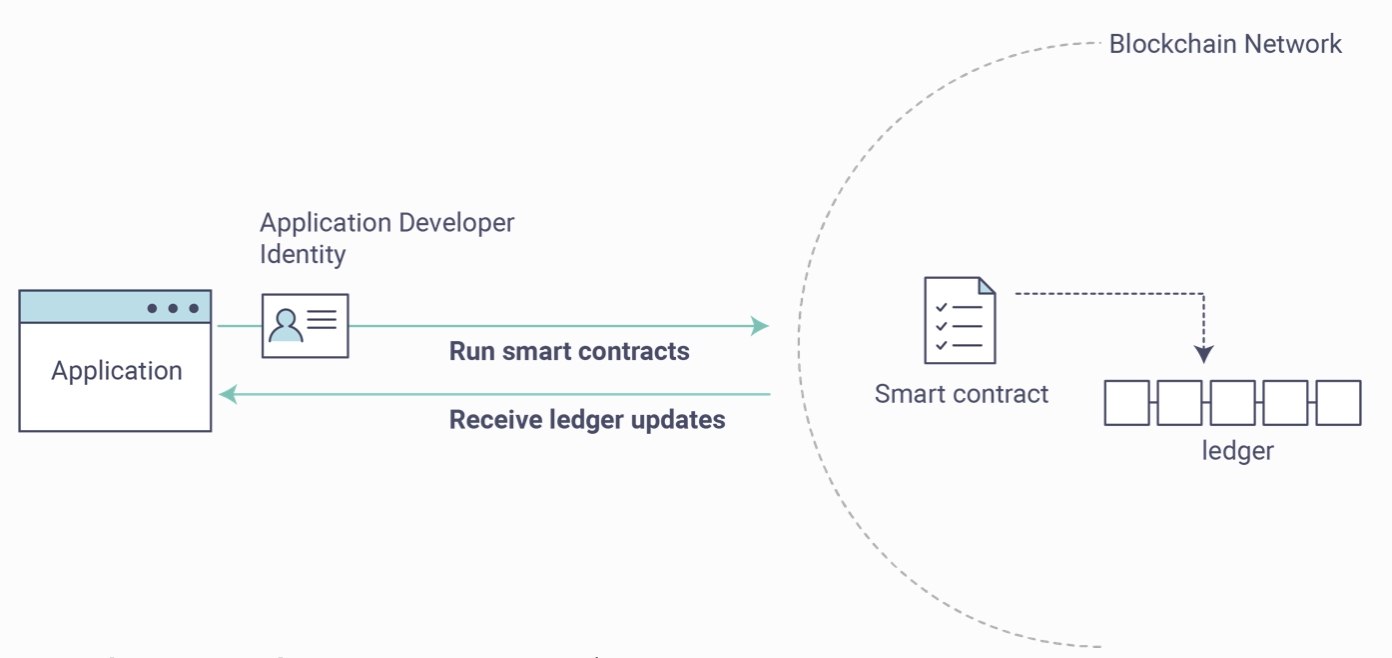
\includegraphics[scale=.4]{app_01}
			\centering
		\end{figure}
		\centering{\tiny{\url{https://hyperledger-fabric.readthedocs.io/en/release-2.0/developapps/application.html}}}
	\end{frame}
	
	\begin{frame}
		\frametitle{Levantar la red blockchain}
		En la ubicación cd fabric-samples/fabcar se levanta la red \textbf{FabCar}
		\begin{center}
			\begin{tabulary}{\linewidth}{L}
				\hline
				\$ ./startFabric.sh javascript \\
				\hline
			\end{tabulary} 
		\end{center}
	\end{frame}
	
	\begin{frame}
		\frametitle{Levantar la red blockchain}
		\textbf{./startFabric.sh javascript} realiza las siguientes tareas:
		\begin{itemize}
			\item Despliega la red \textbf{test-network} de Fabric (2 peer nodes y un ordering service).
			\item Utiliza \textbf{autoridades certificadoras} (CA) para crear los certificados y llaves de la aplicación.
			\item \textbf{Instala el smart contract} de FabCar en el canal mychannel en su versión en JavaScript.
			\item \textbf{Ejecuta el smart contract} para traer los datos iniciales al ledger.
		\end{itemize}
	\end{frame}
	
	\begin{frame}
		\frametitle{Instalar la aplicación}
		En la carpteta cd fabric-samples/fabcar/javascript se encuentran los programas que serán ejecutados por node.js. Para ello hay que instalar las dependencias necesarias.
		\begin{center}
			\begin{tabulary}{\linewidth}{L}
				\hline
				\$ npm install \\
				\hline
			\end{tabulary} 
		\end{center}
	\end{frame}
	
	\begin{frame}
		\frametitle{Usuario administrador}
		Se debe generar la llave pública, la llave privada y el certificado X.509 para admin utilizando el programa enroll.js. Este proceso utiliza una \textbf{Solicitud de firma de certificado}, primero se generan las llaves públicas y privadas de manera local y luego se envía la llave pública a la CA, la cual regresa un certificado codificado para ser usado por la aplicación. 
		\begin{center}
			\begin{tabulary}{\linewidth}{L}
				\hline
				\$ node enrollAdmin.js \\
				\hline
				\$ ls wallet/ \\
				\hline
			\end{tabulary} 
		\end{center}
	\end{frame}

	\begin{frame}
		\frametitle{Usuario cliente}
		Ahora hay que crear una aplicación cliente para interactuar con la blockchain. 
		\begin{center}
			\begin{tabulary}{\linewidth}{L}
				\hline
				\$ node registerUser.js \\
				\hline
				\$ ls wallet/ \\
				\hline
			\end{tabulary} 
		\end{center}
	\end{frame}

	\begin{frame}
		\frametitle{Solicitar el ledger}
		\begin{figure}[h]
			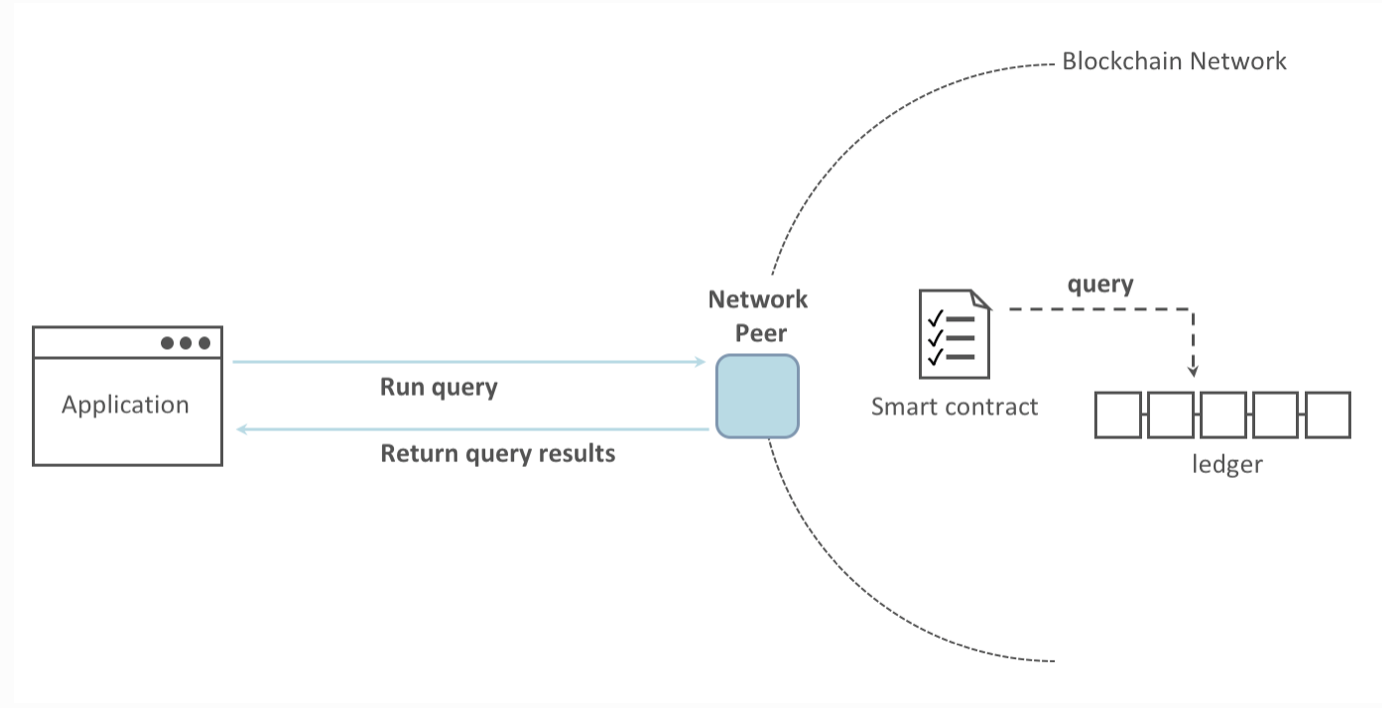
\includegraphics[scale=.4]{app_02}
			\centering
		\end{figure}
		Los valores actuales del ledger están en el \textbf{world state}. El world state está representado como un conjunto llave-valor.
	\end{frame}
	
	\begin{frame}
		\frametitle{Aplicación cliente}
		El usuario appUser realiza la solicitud de todos los carros del ledger.
		\begin{center}
			\begin{tabulary}{\linewidth}{L}
				\hline
				\$ node query.js \\
				\hline
			\end{tabulary} 
		\end{center}
		\begin{figure}[h]
			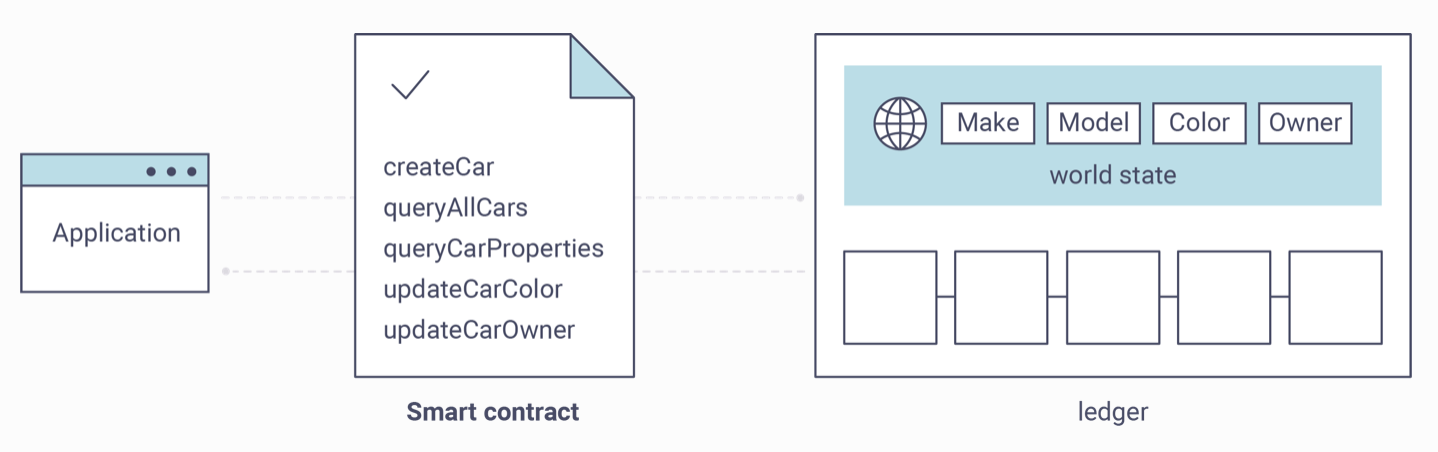
\includegraphics[scale=.4]{app_03}
			\centering
		\end{figure}
	\end{frame}
	
	\begin{frame}
		\frametitle{Contrato FabCar}
		En cd fabric-samples/chaincode/fabcar/javascript/lib se puede ver el smart contract de FabCar.
		\begin{center}
			\begin{tabulary}{\linewidth}{L}
				\hline
				\$ code fabcar.js \\
				\hline
			\end{tabulary} 
		\end{center}
	\end{frame}
	
	\begin{frame}
		\frametitle{Actualizar el ledger}
		\begin{figure}[h]
			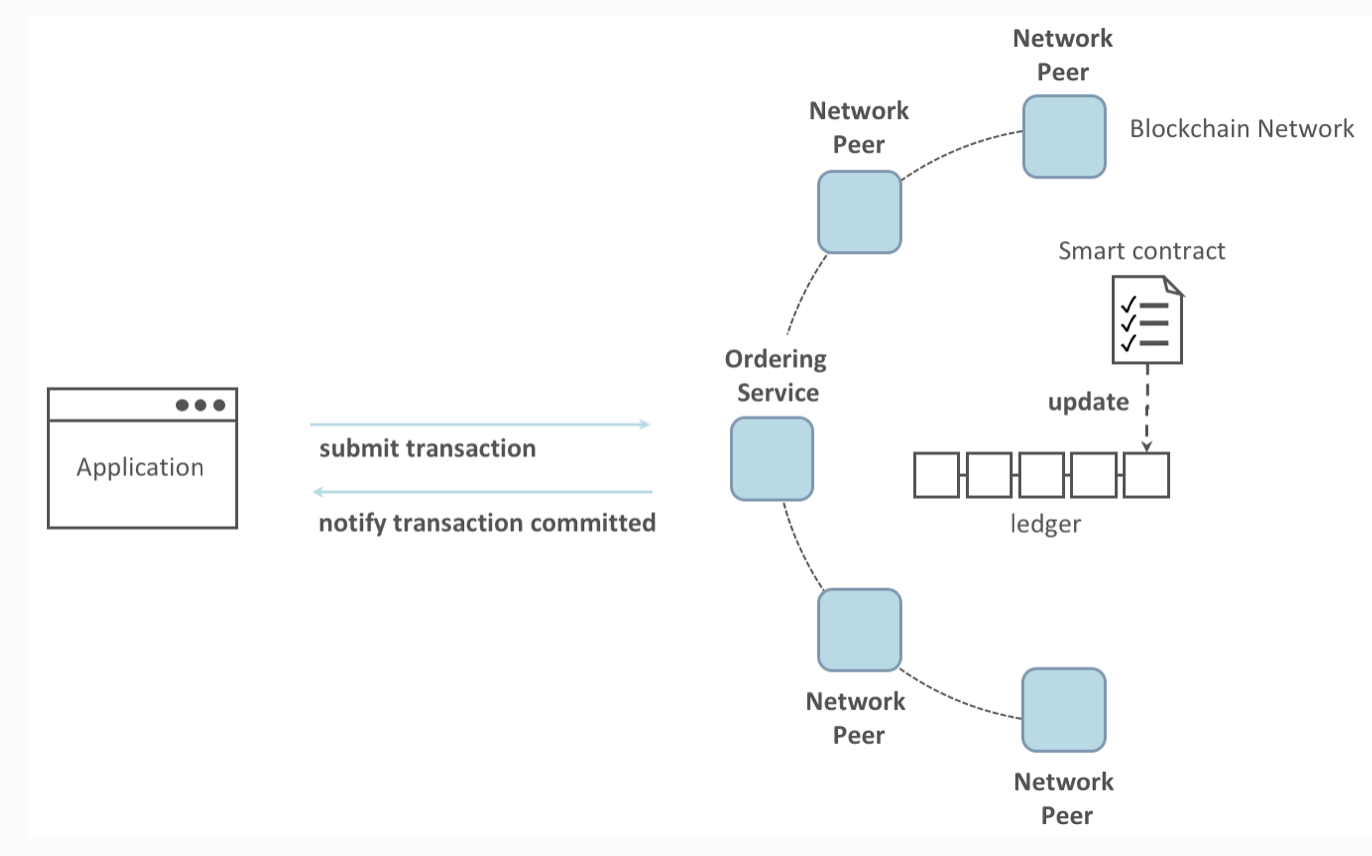
\includegraphics[scale=.4]{app_04}
			\centering
		\end{figure}
	\end{frame}

	\begin{frame}
		\frametitle{Crear un nuevo carro}
		Vamos a crear un nuevo carro, para ello en cd fabric-samples/fabcar/javascript se tiene el programa invoke.js.
		\begin{center}
			\begin{tabulary}{\linewidth}{L}
				\hline
				\$ code invoke.js \\
				\hline
				\$ node invoke.js \\
				\hline
			\end{tabulary} 
		\end{center}
	\end{frame}
	
	\begin{frame}
		\frametitle{Cambio de dueño}
		Vamos a cambiar de dueño al nuevo carro que se creó, para ello en cd fabric-samples/fabcar/javascript se tiene el programa invoke.js en lugar de createCar se invocará changeCarOwner.
		\begin{center}
			\begin{tabulary}{\linewidth}{L}
				\hline
				\$ await contract.submitTransaction('changeCarOwner', 'CAR12', 'Dave'); \\
				\hline
				\$ node invoke.js \\
				\hline
			\end{tabulary} 
		\end{center}
	\end{frame}
	
	\begin{frame}
		\frametitle{Limpiar}
		Para terminar en cd fabric-samples/fabcar, es necesario dar de baja la red, las CA, los nodos peer y ordering y eliminar los wallet de usuario y administrador.
		\begin{center}
			\begin{tabulary}{\linewidth}{L}
				\hline
				\$ ./networkDown.sh \\
				\hline
			\end{tabulary} 
		\end{center}
	\end{frame}
	
	\begin{frame}
		\frametitle{Referencia}
		\begin{center}
			\url{https://hyperledger-fabric.readthedocs.io/en/release-2.0/write_first_app.html}
		\end{center}
	\end{frame}
	
	\section{Papel comercial}
	
	\begin{frame}
		Diagrama de las organizaciones:
		\begin{figure}[h]
			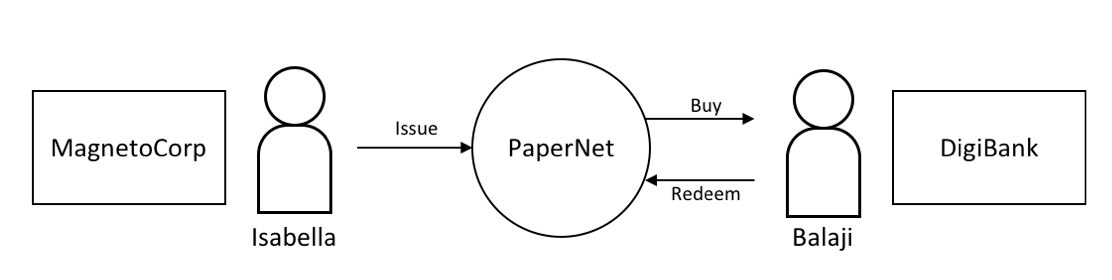
\includegraphics[scale=.5]{papernet_01}
			\centering
		\end{figure}
		Las organizaciones MagnetoCorp y DigiBank intercambian \textbf{papeles comerciales} en la red \textbf{PaperNet}.
	\end{frame}
	
	\subsection{PaperNet}

	\begin{frame}
		\frametitle{Peers y canal de comunicación}
		\begin{figure}[h]
			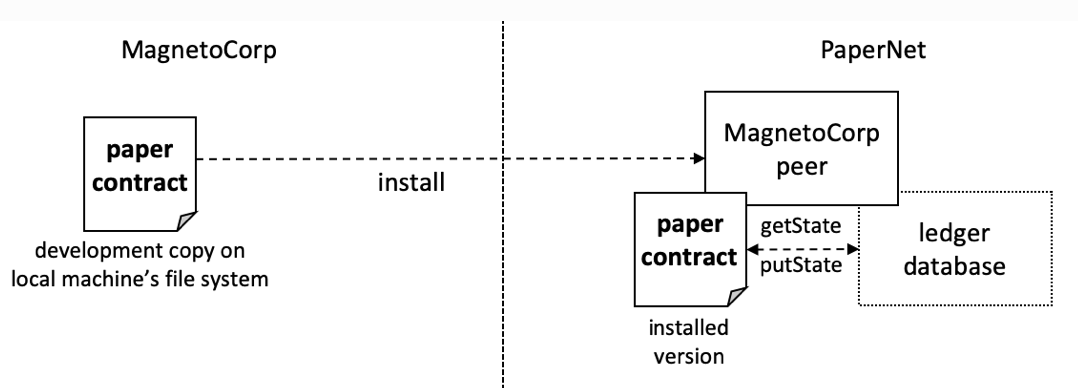
\includegraphics[scale=.5]{papernet_02}
			\centering
		\end{figure}
	\end{frame}
	
	\begin{frame}
		\frametitle{Red docker net\_test}
		En cd fabric-samples/commercial-paper\\
		\begin{center}
			\begin{tabulary}{\linewidth}{L}
				\hline
				(PaperNet admin)\$ ./network-starter.sh \\
				\hline 
				(PaperNet admin)\$ docker ps \\
				\hline
				(PaperNet admin)\$ docker network inspect net\_test \\
				\hline
			\end{tabulary} 
		\end{center}
		peer0.org1.example.com $\rightarrow$ DigiBank\\
		peer0.org2.example.com $\rightarrow$ MagnetoCorp
	\end{frame}
	
	\begin{frame}
		\frametitle{Red docker net\_test}
		Es importante validar que en la variable PATH se encuentre la carpeta \textbf{bin} de fabric-samples y que en la variable FABRIC\_CFG\_PATH se encuentre la carpeta \textbf{config}.
		\begin{center}
			\begin{tabulary}{\linewidth}{L}
				\hline
				(PaperNet admin)\$ export PATH=\${PWD}/../bin:\${PWD}:\$PATH\\
				\hline
				(PaperNet admin)\$ export FABRIC\_CFG\_PATH=\$PWD/../config/\\
				\hline
			\end{tabulary} 
		\end{center}
	\end{frame}
	
	\begin{frame}
		\frametitle{Monitor de la red}
		Tanto el administrador de la red, como los administradores de cada organización pueden revisar la bitácora de actividades de la red constantemente. Ahora jugaremos el rol de Administrador de MagnetoCorp para monitorear la red, cd commercial-paper/organization/magnetocorp ejecutar:\\
		\begin{center}
			\begin{tabulary}{\linewidth}{L}
				\hline
				(MagnetoCorp admin)\$ ./configuration/cli/monitordocker.sh net\_test \\
				\hline
			\end{tabulary} 
		\end{center}
	\end{frame}
	
	\subsection{Crear smart contract propio (MagnetoCorp)}
	
	\begin{frame}
		\frametitle{Creación del contrato}
		En cd commercial-paper/organization/magnetocorp\\
		\begin{center}
			\begin{tabulary}{\linewidth}{L}
				\hline
				(MagnetoCorp dev)\$ code contract \\
				\hline
			\end{tabulary} 
		\end{center}
		Para ver cómo fue diseñado papercontract.js más a detalle se puede consultar:  \small{\url{https://hyperledger-fabric.readthedocs.io/en/release-2.0/developapps/smartcontract.html}}
	\end{frame}

	\begin{frame}
		\frametitle{Ciclo de vida en Fabric}
		\begin{figure}[h]
			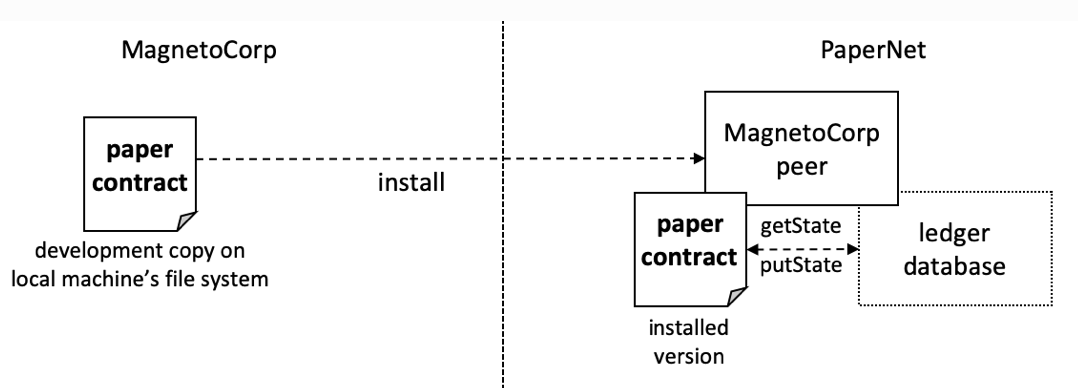
\includegraphics[scale=.4]{papernet_04}
			\centering
		\end{figure}
		\begin{itemize}
			\item Organización emisora
			\begin{itemize}
				\item El desarrollador empaqueta el chaincode ([1...n] smart contract)
				\item El administrador instalar el chaincode en cada organización.
			\end{itemize}
			\item Organización receptora
			\begin{itemize}
				\item El administrador debe aprobar el chaincode.
				\item El administrador publica el chaincode en el ledger del canal asociado.
			\end{itemize}
		\end{itemize}
		{\tiny \url{https://hyperledger-fabric.readthedocs.io/en/release-2.0/chaincode\_lifecycle.html\#chaincode-lifecycle} }
	\end{frame}
	
	\begin{frame}
		\frametitle{Instalación}
		\textbf{Variables de entorno:} En cd commercial-paper/organization/magnetocorp hay que establecer las variables de entorno para que el administrador pueda instalar y aprobar el chaincode en la organización MagnetoCorp.\\
		\begin{center}
			\begin{tabulary}{\linewidth}{L}
				\hline
				(MagnetoCorp admin)\$ source magnetocorp.sh \\
				\hline
			\end{tabulary} 
		\end{center}
	\end{frame}
	
	\begin{frame}
		\frametitle{Instalación}
		\textbf{Empaquetar el chaincode:} Para instalar el contrato, primero se debe empaquetar el smart contract en un chaincode.\\
		\begin{center}
			\begin{tabulary}{\linewidth}{L}
				\hline
				(MagnetoCorp admin)\$ peer lifecycle chaincode package cp.tar.gz - -lang node - -path ./contract - -label cp\_0\\
				\hline
			\end{tabulary} 
		\end{center}
	\end{frame}
	
	\begin{frame}
		\frametitle{Instalación}
		\textbf{Instalar el chaincode:} Una vez generado el paquete se puede instalar en el peer node de la organización.\\
		\begin{center}
			\begin{tabulary}{\linewidth}{L}
				\hline
				(MagnetoCorp admin)\$ peer lifecycle chaincode install cp.tar.gz\\
				\hline
			\end{tabulary} 
		\end{center}
	\end{frame}
	
	\begin{frame}
		\frametitle{Aprobación}
		\textbf{Package ID:} Para poder aprobar el contrato primero se debe obtener el packageID del chaincode que se acaba de instalar.\\
		\begin{center}
			\begin{tabulary}{\linewidth}{L}
				\hline
				(MagnetoCorp admin)\$ peer lifecycle chaincode queryinstalled \\
				\hline
			\end{tabulary} 
		\end{center}
	\end{frame}
	
	\begin{frame}
		\frametitle{Aprobación}
		\textbf{Guardar el package ID:} El package ID se va a ocupar en el siguiente paso, se puede guardar en una variable de entorno.\\
		\begin{center}
			\begin{tabulary}{\linewidth}{L}
				\hline
				(MagnetoCorp admin)\$ export PACKAGE\_ID=cp\_0:ffda9... \\
				\hline
			\end{tabulary} 
		\end{center}
	\end{frame}
	
	\begin{frame}
		\frametitle{Aprobación}
		\textbf{Aprobar el chaincode:} El administrador de MagnetoCorp debe aprobar el papercontract.\\
		\begin{center}
			\begin{tabulary}{\linewidth}{L}
				\hline
				(MagnetoCorp admin)\$ peer lifecycle chaincode approveformyorg - -orderer localhost:7050 - -ordererTLSHostnameOverride orderer.example.com - -channelID mychannel - -name papercontract -v 0 - -package-id \$PACKAGE\_ID - -sequence 1 - -tls - -cafile \$ORDERER\_CA \\
				\hline
			\end{tabulary} 
		\end{center}
	\end{frame}

	\begin{frame}
		\frametitle{Aprobación}
		La política de aprobación define el número de organizaciones que debe endosar (ejecutar y firmar) una transacción antes de determinarse como válida.\\
		\vspace{4mm}
		El contrato se aprobó por MagnetoCorp con la política por defecto de la red, la cual requiere que la mayoría de las organizaciones validen la transacción. Todas las transacciones, válidas o inválidas, se guardan en la blockchain, pero solo las válidas modifican el estado (\textbf{world state}).\\
		\centering{\tiny{\url{https://hyperledger-fabric.readthedocs.io/en/release-2.0/ledger/ledger.html}}}
	\end{frame}
	
	\subsection{Aprobar smart contract de terceros (DigiBank)}
	
	\begin{frame}
		\frametitle{Instalación}
		Por defecto, el ciclo de vida del chaincode en Fabric requiere que la mayoría de las organizaciones apruebe la definición de un chaincode en el canal. En este caso, se tienen 2 organizaciones, por lo tanto, se requiere que las 2 organizaciones apruebe el chaincode.
	\end{frame}
	
	\begin{frame}
		\frametitle{Instalación}
		\textbf{Variables de entorno:} En cd commercial-paper/organization/digibank/ hay que establecer las variables de entorno para que el administrador de DigiBank pueda instalar y aprobar el papernet chaincode.\\
		\begin{center}
			\begin{tabulary}{\linewidth}{L}
				\hline
				(DigiBank admin)\$ source digibank.sh\\
				\hline
			\end{tabulary} 
		\end{center}
	\end{frame}
	
	\begin{frame}
		\frametitle{Instalación}
		\textbf{Empaquetar el chaincode:} El smart contract se debe empacar en un chaincode.\\
		\begin{center}
			\begin{tabulary}{\linewidth}{L}
				\hline
				(DigiBank admin)\$ peer lifecycle chaincode package cp.tar.gz - -lang node - -path ./contract - -label cp\_0\\
				\hline
			\end{tabulary} 
		\end{center}
	\end{frame}
	
	\begin{frame}
		\frametitle{Instalación}
		\textbf{Instalar el chaincode:} Ahora se puede instalar el chaincode empaquetado en la organización.\\
		\begin{center}
			\begin{tabulary}{\linewidth}{L}
				\hline
				(DigiBank admin)\$ peer lifecycle chaincode install cp.tar.gz\\
				\hline
			\end{tabulary} 
		\end{center}
	\end{frame}
	
	\begin{frame}
		\frametitle{Aprobación}
		\textbf{Package ID:} Para poder aprobar el contrato primero se debe obtener el packageID del chaincode que se acaba de instalar.\\
		\begin{center}
			\begin{tabulary}{\linewidth}{L}
				\hline
				(DigiBank admin)\$ peer lifecycle chaincode queryinstalled \\
				\hline
			\end{tabulary} 
		\end{center}
	\end{frame}
	
	\begin{frame}
		\frametitle{Aprobación}
		\textbf{Guardar el package ID:} El package ID se va a ocupar en el siguiente paso, se puede guardar en una variable de entorno.\\
		\begin{center}
			\begin{tabulary}{\linewidth}{L}
				\hline
				(DigiBank admin)\$ export PACKAGE\_ID=cp\_0:ffda9... \\
				\hline
			\end{tabulary} 
		\end{center}
	\end{frame}
	
	\begin{frame}
		\frametitle{Aprobación}
		\textbf{Aprobar el chaincode:} El administrador de DigiBank debe aprobar el papercontract.\\
		\begin{center}
			\begin{tabulary}{\linewidth}{L}
				\hline
				(DigiBank admin)\$ peer lifecycle chaincode approveformyorg --orderer localhost:7050 - -ordererTLSHostnameOverride orderer.example.com - -channelID mychannel - -name papercontract -v 0 - -package-id \$PACKAGE\_ID - -sequence 1 - -tls - -cafile \$ORDERER\_CA \\
				\hline
			\end{tabulary} 
		\end{center}
	\end{frame}
	
	\subsection{Publicar smart contract (DigiBank)}
	
	\begin{frame}
		\frametitle{Publicación}
		Una vez que el contrato ha sido aprobado por la mayoría del consorcio (2/2) en el canal, se envía la definición del chaincode al canal.\\
		\vspace{4mm}
		Ahora, el contrato inteligente CommercialPaper puede ser invocado por alguna aplicación cliente en el canal.
	\end{frame}

	\begin{frame}
		\frametitle{Publicación}
		\textbf{Publicar papercontract:} El administrador de cualquier organización puede publicar el smart contract en el canal.\\
		\begin{center}
			\begin{tabulary}{\linewidth}{L}
				\hline
				(DigiBank admin)\$ peer lifecycle chaincode commit -o localhost:7050 - -ordererTLSHostnameOverride orderer.example.com - -peerAddresses localhost:7051 - -tlsRootCertFiles \${PEER0\_ORG1\_CA} - -peerAddresses localhost:9051 - -tlsRootCertFiles \${PEER0\_ORG2\_CA} - -channelID mychannel - -name papercontract -v 0 - -sequence 1 - -tls - -cafile \$ORDERER\_CA - -waitForEvent\\
				\hline
			\end{tabulary} 
		\end{center}
	\end{frame}
	
	\subsection{Emisión de papel comercial (MagnetoCorp)}
	
	\begin{frame}
		\frametitle{Diagrama de emisión}
		MagnetoCorp utiliza su aplicación cliente \textbf{issue.js} y emitir el papel comercial .
		\begin{figure}[h]
			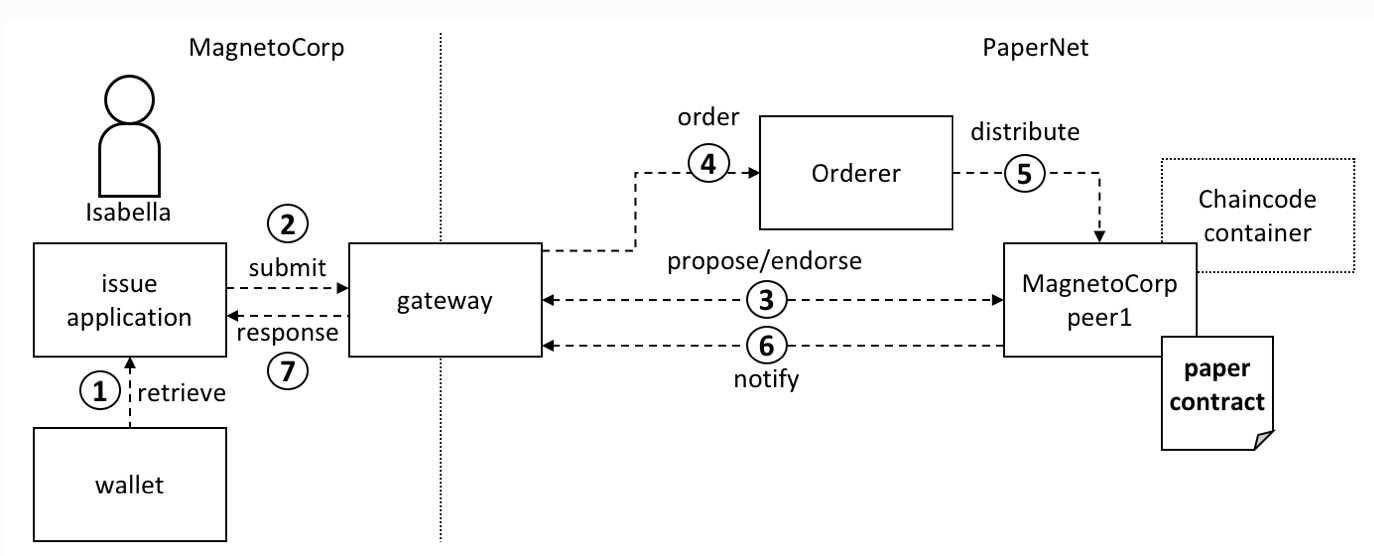
\includegraphics[scale=.4]{papernet_05}
			\centering
		\end{figure}
	\end{frame}
	
	\begin{frame}
		\frametitle{Emisión}
		En cd commercial-paper/organization/magnetocorp/application/ se pueden ver los archivos \textbf{addToWallet.js}, \textbf{issue.js} y \textbf{package.json}.\\
		\vspace{4mm}
		Isabella va a utilizar addToWallet.js para agregar su identidad al wallet (Certificado X.509) y luego issue.js utilizará esa identidad para crear el papel comercial a nombre de MagnetoCorp invocando al papercontract.
	\end{frame}
	
	\begin{frame}
		\frametitle{Emisión}
		La aplicación cliente \textbf{issue.js} está escrita en javascript y se ejecutará en node.js. Los paquetes \textbf{js-yaml} y \textbf{fabric-network} se deben descargar de npm.\\
		\vspace{4mm}
		Los paquetes y las versiones necesarias están declaradas en el archivo \textbf{package.json}.
		\begin{center}
			\begin{tabulary}{\linewidth}{L}
				\hline
				(MagnetoCorp Isabella)\$ npm install \\
				\hline
			\end{tabulary} 
		\end{center}
	\end{frame}

	\begin{frame}
		\frametitle{Emisión}
		Por convención, los paquetes descargados por \textbf{npm} se guardan en la carpeta \textbf{/node\_modules}, donde se ejecutó el comando.
		\begin{center}
			\begin{tabulary}{\linewidth}{L}
				\hline
				(MagnetoCorp Isabella)\$ ls \\
				\hline
			\end{tabulary} 
		\end{center}
	\end{frame}
	
	\begin{frame}
		\frametitle{Emisión}
		Para que Isabella pueda ejecutar emitir el papel comercial \textbf{00001}, se deben agregar su credenciales X.509 a su wallet.\\
		\begin{center}
			\begin{tabulary}{\linewidth}{L}
				\hline
				(MagnetoCorp Isabella)\$ node addToWallet.js \\
				\hline
				(MagnetoCorp Isabella)\$ ls ../identity/user/isabella/wallet/ \\
				\hline
			\end{tabulary} 
		\end{center}
	\end{frame}
	
	\begin{frame}
		\frametitle{Emisión}
		Ahora sí, Isabella puede utilizar \textbf{issue.js} para enviar la transacción que emitirá el papel comercial \textbf{00001} de parte de MagnetoCorp.\\
		\begin{center}
			\begin{tabulary}{\linewidth}{L}
				\hline
				(Isabella)\$ node issue.js \\
				\hline
			\end{tabulary} 
		\end{center}
	\end{frame}
	
	\subsection{Comprar un papel comercial (DigiBank)}
	
	\begin{frame}
		\frametitle{Compra}
		Para comprar el papel comercial que emitió MagnetoCorp, el usuario de DigiBank (Balaji) debe realizar una transacción de compra desde la aplicación de DigiBank.
	\end{frame}
	
	\begin{frame}
		\frametitle{Compra}
		En cd commercial-paper/organization/digibank/application/ se pueden ver los archivos \textbf{addToWallet.js}, \textbf{buy.js}, \textbf{package.json} y \textbf{redeem.js}\\
		\vspace{4mm}
		Balaji va a utilizar buy.js y redeem.js para comprar y, posteriormente, canjear el papel comercial que emitió MagnetoCorp.
	\end{frame}
	
	\begin{frame}
		\frametitle{Compra}
		Al igual que en MagnetoCorp, DigiBank debe instalar los paquetes declarados en \textbf{package.json} a través de npm.\\
		\begin{center}
			\begin{tabulary}{\linewidth}{L}
				\hline
				(Balaji)\$ npm install \\
				\hline
			\end{tabulary} 
		\end{center}
	\end{frame}
	
	\begin{frame}
		\frametitle{Compra}
		Para que Balaji pueda comprar el papel comercial, debe agregar sus identidad a su wallet ejecutando el programa \textbf{addToWallet.js}.\\
		\begin{center}
			\begin{tabulary}{\linewidth}{L}
				\hline
				(Balaji)\$ node addToWallet.js \\
				\hline
			\end{tabulary} 
		\end{center}
	\end{frame}
	
	\begin{frame}
		\frametitle{Compra}
		Finalmente, Balaji puede enviar la transacción \textbf{buy.js} para transferir (comprar) el papel comercial de MagnetoCorp a DigiBank.\\
		\begin{center}
			\begin{tabulary}{\linewidth}{L}
				\hline
				(Balaji)\$ node buy.js \\
				\hline
			\end{tabulary} 
		\end{center}
	\end{frame}
	
	\subsection{Canjear el papel comercial (DigiBank)}
	
	\begin{frame}
		\frametitle{Canjear}
		La transacción final para el papel comercial \textbf{00001} será que DigiBank lo intercambie con MagnetoCorp. Para ello Balaji utilizará el \textbf{redeem.js}.\\
		\begin{center}
			\begin{tabulary}{\linewidth}{L}
				\hline
				(Balaji)\$ node redeem.js \\
				\hline
			\end{tabulary} 
		\end{center}
	\end{frame}
	
	\subsection{Limpiar el proyecto}
	
	\begin{frame}
		\frametitle{Limpiar}
		En cd fabric-samples/commercial-paper.\\
		\begin{center}
			\begin{tabulary}{\linewidth}{L}
				\hline
				(Balaji)\$ ./network-clean.sh \\
				\hline
			\end{tabulary} 
		\end{center}
		Este script dará de baja los peers, los contenedores, el nodo ordering service y el logspout. Además, eliminará las identidades de Isabella y Balaji.
	\end{frame}
	
	\begin{frame}
		\frametitle{Referencia}
		\begin{center}
			\url{https://hyperledger-fabric.readthedocs.io/en/release-2.0/tutorial/commercial\_paper.html}
		\end{center}
	\end{frame}
\end{document}